\documentclass[tikz,border=5pt]{standalone}
\usepackage[T1]{fontenc}
\usepackage{lmodern,amsmath,amssymb}
\usetikzlibrary{arrows.meta,calc,positioning,fit,backgrounds,shapes.geometric,matrix,decorations.pathreplacing,patterns}
\definecolor{ink}{gray}{0.08}
\definecolor{wash}{gray}{0.965}
\definecolor{soft}{gray}{0.45}
\tikzset{box/.style={draw=ink,line width=.65pt,fill=white,align=center,inner sep=4pt,outer sep=0pt,font=\small},flow/.style={draw=ink,line width=.65pt,-{Latex[length=1.8mm,width=1.3mm]},rounded corners=2pt},annotation/.style={font=\scriptsize,text=soft,align=center},groupbox/.style={draw=soft,dashed,line width=.45pt,fill=wash}}
\begin{document}
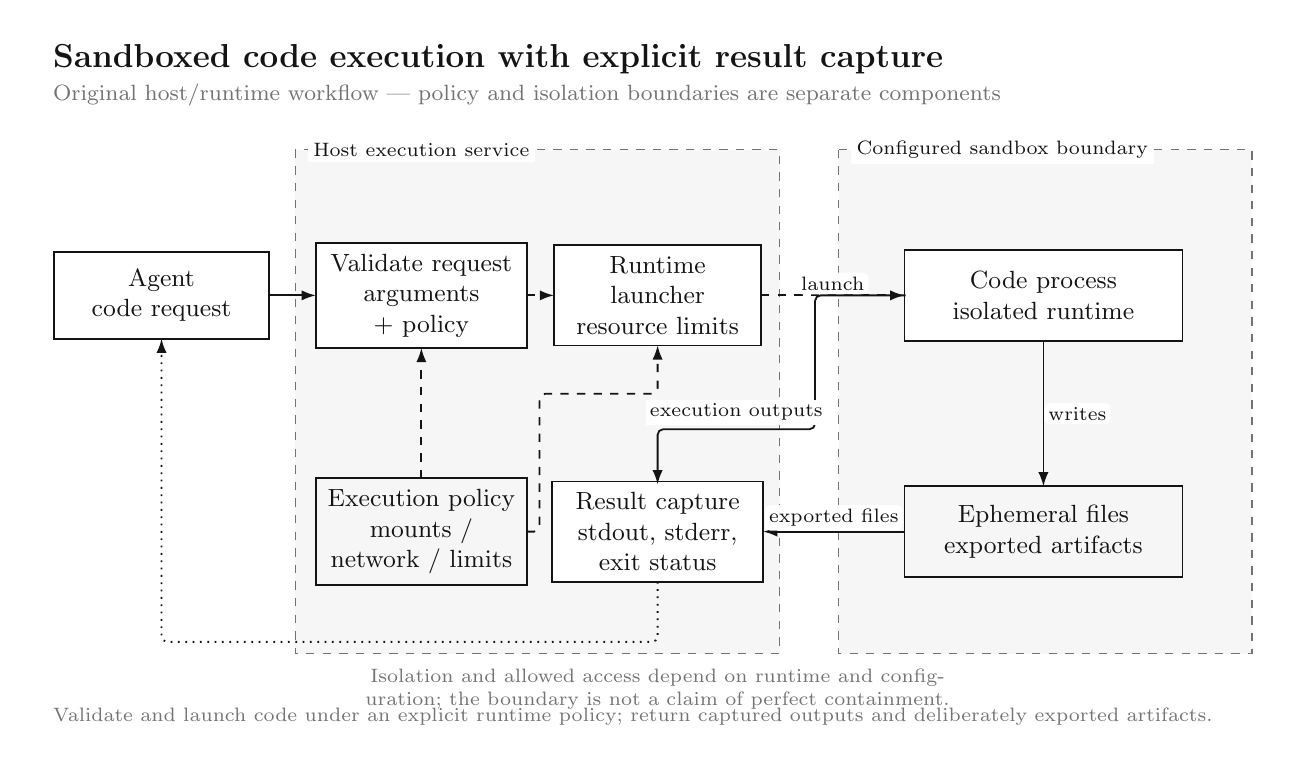
\begin{tikzpicture}[x=1cm,y=-1cm,font=\rmfamily,text=ink]

\path[use as bounding box] (0,0) rectangle (16,9);
\node[anchor=west,font=\large\bfseries] at (.2,.4) {Sandboxed code execution with explicit result capture};
\node[anchor=west,font=\footnotesize,text=soft] at (.2,.85) {Original host/runtime workflow | policy and isolation boundaries are separate components};
\begin{pgfonlayer}{background}
\draw[groupbox] (3.4,1.55) rectangle (9.55,7.95);
\node[anchor=west,font=\scriptsize,fill=white,inner sep=2pt] at (3.55,1.55) {Host execution service};
\draw[groupbox] (10.3,1.55) rectangle (15.55,7.95);
\node[anchor=west,font=\scriptsize,fill=white,inner sep=2pt] at (10.450000000000001,1.55) {Configured sandbox boundary};
\end{pgfonlayer}
\node[box,minimum width=2.7cm,minimum height=1.1cm,text width=2.45cm] (agent) at (1.7,3.4) {Agent\\code request};
\node[box,minimum width=2.65cm,minimum height=1.1cm,text width=2.4cm] (validate) at (5.0,3.4) {Validate request\\arguments + policy};
\node[box,minimum width=2.6cm,minimum height=1.1cm,text width=2.35cm] (launch) at (8.0,3.4) {Runtime launcher\\resource limits};
\node[box,minimum width=3.5cm,minimum height=1.15cm,text width=3.25cm] (process) at (12.9,3.4) {Code process\\isolated runtime};
\node[box,fill=wash,minimum width=2.65cm,minimum height=1.2cm,text width=2.4cm] (policy) at (5.0,6.4) {Execution policy\\mounts / network / limits};
\node[box,minimum width=2.65cm,minimum height=1.2cm,text width=2.4cm] (capture) at (8.0,6.4) {Result capture\\stdout, stderr, exit status};
\node[box,fill=wash,minimum width=3.5cm,minimum height=1.15cm,text width=3.25cm] (files) at (12.9,6.4) {Ephemeral files\\exported artifacts};
\begin{pgfonlayer}{background}
\draw[flow] (agent.east) -- (validate.west);
\draw[flow,dashed] (validate.east) -- (launch.west);
\draw[flow,dashed] (launch.east) -- (process.west) node[midway,above,fill=white,inner sep=1.5pt,font=\scriptsize] {launch};
\draw[flow,dashed] (policy.north) -- (validate.south);
\draw[flow,dashed] (policy.east) -- (6.5,6.4) -- (6.5,4.65) -- (8,4.65) -- (launch.south);
\draw[flow] (process.south) -- (files.north) node[midway,right,fill=white,inner sep=1.5pt,font=\scriptsize] {writes};
\draw[flow] (files.west) -- (capture.east) node[midway,above,fill=white,inner sep=1.5pt,font=\scriptsize] {exported files};
\draw[flow,dotted] (capture.south) -- (8,7.8) -- (1.7,7.8) -- (agent.south);
\end{pgfonlayer}
\draw[flow] (11.15,3.4) -- (10.0,3.4) -- (10.0,5.1) -- (8.0,5.1) -- (8.0,5.8);
\node[font=\scriptsize,fill=white,inner sep=1.5pt,anchor=south] at (9.0,5.05) {execution outputs};
\node[annotation,anchor=center,text width=14.5cm] at (8,8.4) {Isolation and allowed access depend on runtime and configuration; the boundary is not a claim of perfect containment.};
\node[anchor=west,align=left,font=\scriptsize,text=soft,text width=15.6cm] at (.2,8.75) {Validate and launch code under an explicit runtime policy; return captured outputs and deliberately exported artifacts.};
\end{tikzpicture}
\end{document}
